\chapter{Einleitung und Aufgabenstellung}


\section{Einleitung}
Der Blutkreislauf ist eine der wichtigsten Regeleinrichtungen des menschlichen Organismus. Dieser Kreislauf transportiert Blut, welches sich aus festen - Erythrozyten, Leukozyten und Thrombozyten - und flüssigen - Plasma - Bestandteilen zusammensetzt. Dabei passt sich der Kreislauf an die aktuelle Belastungsart an, indem er die Durchflussgeschwindigkeit des Blutes reguliert. Jedoch ist die Durchflussgeschwindigkeit durch die Herzfrequenz und den Arterienquerschnitten begrenzt.
%Arterien können durch die erhöhte bzw. ungesunde Zufuhr von Nahrungsmitteln sowie Genussmitteln stark belastet werden, da sich Ablagerungen (Gefäßverengung) bilden können oder die Dehnbarkeit der Arterien und somit der maximale Querschnitt reduziert werden kann. 
Dabei kann der Blutfluss durch Ereignisse, sogenannte Embolien, welche in den Gefäßen auftreten gehemmt oder gar zum erliegen gebracht werden. Die Folge ist ein minderperfundiertes betroffenes Gewebe mit anschließenden Absterben von Zellen. Dabei gibt es drei Emboliearten, welche primär in der ambulanten und stationären Behandlung vorherrschen und ein Zellsterben mit sich bringen.
\begin{description}
\item[Luft- / Gasembolie] welche durch Injektion von Gas oder bei schnellen auftauchen aus großen Tiefen\footnote{Taucher- bzw. Dekompressionskrankheit} entstehen können. Injektionen treten meist bei Operationen am offenen Herzen und bei Operationen an Arterien auf.
\item[Tromboembolie] umgangssprachlich auch \glqq Blutgerinnsel\grqq{} genannt, entsteht durch eine Ansammlung von Blutblättchen an der Gefäßwand, welche durch Arterienverkalkungen begünstigt werden kann. Diese Ansammlung kann sich von der Gefäßwand lösen und anschließend die Arterie verschließen.
\item[Fettembolie] ist eine Ansammlung von Fetttröpfchen bzw. Fettzellen, welche nach offenen Knochenbrüchen in den Blutkreislauf eingeschwemmt werden können.
\end{description}
Da diese Ereignisse vermehrt zufällig auftreten und das Risiko mitunter von dem Patienten abhängig ist, wurde für Lungenembolien der Wells-Score nach dem Wissenschaftler P.S. Wells eingeführt. Dieser Score beschreibt die Dringlichkeit und den zu betreibenden Aufwand für eine Diagnose. Des weiteren ist bekannt, dass bei Operationen vermehrt Ereignisse auftreten können, welche jedoch durch die relaxierte Muskulatur des Patienten nur bedingt wahrgenommen werden kann. Ein Monitoring zentraler Arterien während der Patient narkotisiert ist, könnte Embolien aufdecken und somit ein schnelle Entscheidungsfindung bei Schlaganfällen oder Lungenembolien begünstigen.\\
Die zeitnahe Erkennung von Ereignissen ist somit von zentraler Bedeutung für jeden behandelnden Arzt, da in der operativen Medizin jeder Zeit -  \glqq Time is Brain\grqq{}, \glqq Time is Muscle\grqq{} und \glqq Golden hour\footnote{Zeit zum verhindern schlimmerer Sachen}\grqq{} - Komplikationen auftreten können. Die Erkennung eines Ereignisses erlaubt es dem Arzt zu entscheiden, ob die Operation weitergeführt werden kann oder abgebrochen werden muss. Dabei hat ein Abbruch der Operation eine Lysetherapie mit einer erhöhten Dosis Heparin gegen die erkannte Embolie zur Folge.\\
Ein Monitoring von Ereignissen sollte an den Hauptarterien durchgeführt werden, da diese einen erhöhten Volumenstrom und somit eine erhöhte Chance auf die Erkennung von Ereignissen bieten. Dabei sind invasive\footnote{latein invadere \textit{einfallen, eindringen}} Methoden nicht zu empfehlen, da diese Gewebeschäden zur Folge haben. Eine Alternative bieten nicht invasive Methoden, da diese den Patienten nicht verletzen und das Gewebe zerstören wodurch eine Beobachtung von Gehirnarterien ermöglicht werden kann.\\
Die vorliegende Arbeit befasst sich aus diesem Grund mit der Umsetzung einer nicht invasiven Methode zur schnellen und eindeutigen Emboliedetektion.

\section{Aufgabenstellung}
\subsection{Aufgabenstellung der Masterarbeit}
Ziel dieser Arbeit ist die Realisierung eines Systems für die eindeutige Detektion von Embolien auf Basis der nichtinvasiven gepulsten Ultraschall-Dopplertechnologie. Eine Visualisierung in Spektrogramm und M-Mode sowie die akustische Wiedergabe der Signale sind dabei unverzichtbar, um möglichst viele Informationen aus der zeitnahen Messung zu generieren und somit eine eindeutige Detektion zu gewährleisten. \autoref{fig:usdschema} visualisiert dabei das grundlegende Vorhaben.\\
Diese Thesis soll \ac{ua} eine Optimierung einer vorhandenen Hardware darstellen, da eine Detektion von Ereignissen durch die Messgenauigkeit des Messsystems bedingt ist. Beim Designen der Elektronik ist darauf zu achten, dass verschiedene Ultraschallsonden verwendet werden können. Des Weiteren soll eine Optimierung der bereits entwickelten Schnittstelle zum \ac{pc} erfolgen, da die aktuelle Datentransferrate für eine eindeutige Detektion von Embolien nicht ideal erscheint. Zudem muss ein Algorithmus implementiert werden, um Embolien eindeutig zu detektieren und dem Nutzer zu visualisieren. Die Visualisierung der Messung soll dabei auf einen \ac{pc} unter Nutzung diverser Betriebssysteme erfolgen indem eine benutzerfreundliche \ac{gui} bereitgestellt wird. Alle weiteren Details werden in \autoref{sec:sysreq} spezifiziert.
\begin{figure}[ht]
	\centering
	\begin{subfigure}[b]{0.48\textwidth}
		\centering
  		\includegraphics[page=2, trim = 16mm 22mm 97mm 216mm, clip=true, width=0.7\textwidth]{Ultrasound/Embolusdetection_tutorial}  
		\caption{Transcraniale Emitierung von Ultraschall}
  	\end{subfigure}
  	\hfill
  	\begin{subfigure}[b]{0.48\textwidth}
	  	\centering
  		\includegraphics[page=2, trim = 98mm 237mm 7mm 21mm, clip=true, width=1\textwidth]{Ultrasound/Embolusdetection_tutorial}
	  	\caption{Verarbeitung des Signals}
  	\end{subfigure}
	\caption[Vereinfachte Darstellung der Emboliedetektion]{Vereinfachte Darstellung der Emboliedetektion\cite[p. 2]{emboli}}
  	\label{fig:usdschema}
\end{figure}
%
%
%

\subsection{Vorstellung des vorhandenen Systems}
\subsubsection*{Das digitale Ultraschall-Multigate-Doppler System - Version 2012}\label{cp:usdV1}

Herr Sebastian Stemplewitz entwickelte in seiner Bachelorarbeit an der Hochschule Ulm einen Prototypen für die \ac{pc} gestützte Hämatokritwertmessung. Dieser sollte eine kostengünstige und intravasale Alternative zur aktuellen Hämatokritwertbestimmung werden.\\
Das System ist soweit minimalisiert sowie miniaturisiert(\autoref{fig:system_stemp}), dass eine Weiterentwicklung des Systems die logische Schlussfolge war. Messdaten können erfolgreich mit 8 MHz Sonden aufgenommen und darstellen werden. Dabei dient ein PIC18F4550 \ac{mcu} der Firma Microchip als Schnittstelle zwischen der Messsteuerung und dem \ac{pc} durch die Implementierung eines \ac{usb} Audio-Profils, welches mit der selbst entwickelten Software\footnote{auf Basis von C++ und QT} kommuniziert. Jedoch wurde in der Testphase festgestellt, dass eine Optimierung der Transmitter- und Receiverschaltung notwendig ist um Artefakte zu reduzieren und die Messgenauigkeit zu erhöhen. Aus dem Wunsch, die Kompatibilität mit 2 und 4 MHz Ultraschallsonden zu gewährleisten, entstand die Idee dieses System mit einen ARM-Cortex \ac{mcu} zu betreiben und die Datenverarbeitung und Darstellung über diesen bereitzustellen.\cite{stemp2012}
\newpage
\begin{figure}[h]
\centering
  	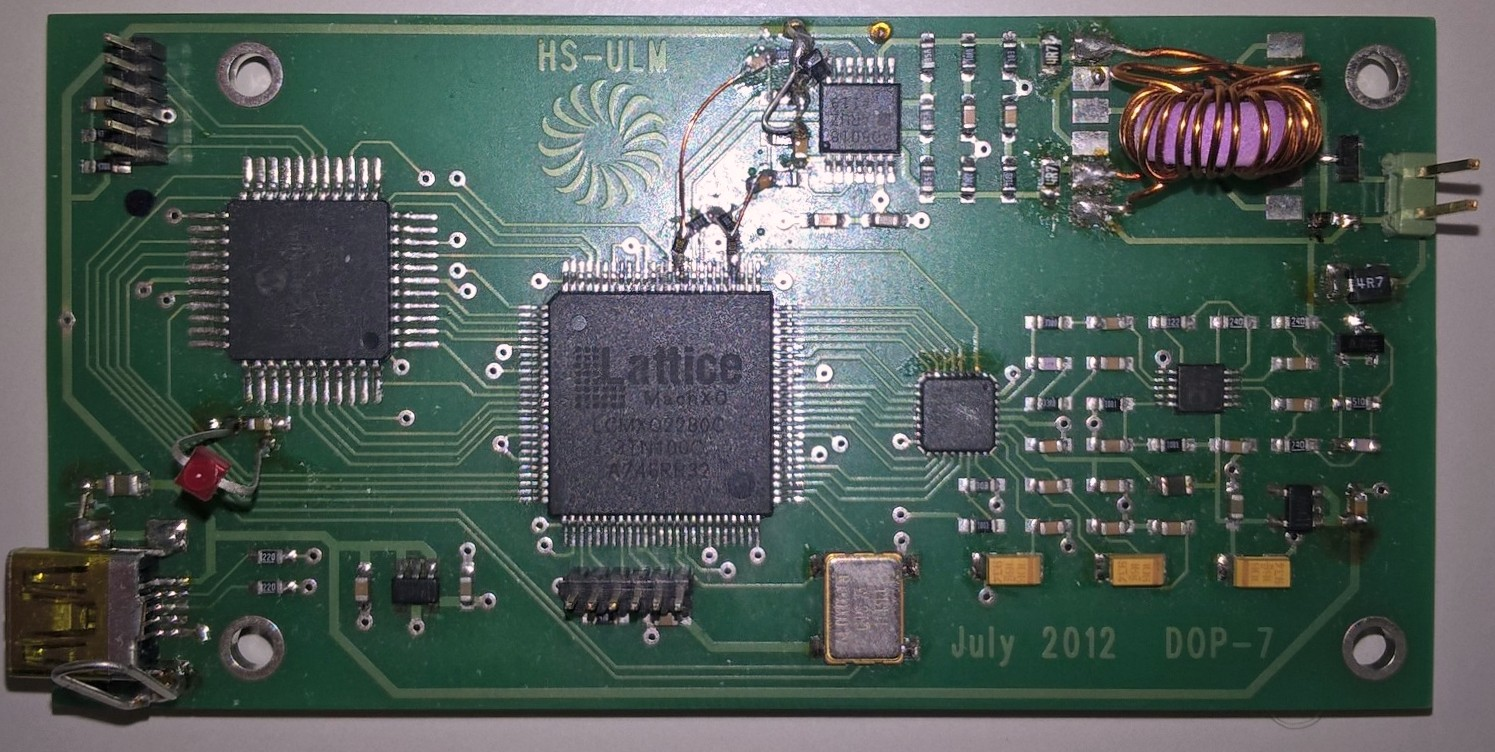
\includegraphics[width=\textwidth]{systemV1}  
	\caption{Systemaufbau Thesis Stemplewitz}
  	\label{fig:system_stemp}
\end{figure}
\begin{table}[h]
\centering
\caption{Bestandteile der Platine}
\label{tab:system_stemp_tab}
\begin{tabular}{c|l}
\textbf{Nr.} & \textbf{Beschreibung} \\
\cline{1-2}
1 & \ac{mcu} und \ac{usb}-Kommunikation\\ 
2 & Signalerzeugung und Dempdulation \ac{cpld}\\ 
3 & Transmitter mit Differenzverstärker und Übertrager\\ 
4 & Receiver mit Vorverstärker und \ac{adc}\\ 
\end{tabular}
\end{table}

\subsubsection*{Das digitale Ultraschall-Multigate-Doppler System - Version 2014}\label{cp:usdV2}
Herr Andreas Rehn, Autor dieser Arbeit, optimierte in seiner Bachelorarbeit an der Hochschule Ulm die Version 2012 (\autoref{cp:usdV1}) für die Hämatokritwertmessung. Dabei wurde das Messsystem modularisiert und ein ARM-Cortex M3 \ac{mcu} für den Datentransfer sowie für die Ansteuerung eines LCD-Displays integriert. Dabei stellte sich heraus, dass das vorhandene \ac{cpld} für die mathematische Vorverarbeitung der Signale keine Reserven bietet. Außerdem konnte eine Steigerung der Flexibilität durch die Umstrukturierung des Zustandsautomaten erreicht werden. Die Datentransferrate zwischen \ac{cpld} und \ac{mcu} wurde auf 15,7 Mbit/s gesteigert, welche durch das \ac{usb} Full-Speed Interface auf 12 Mbit/s (brutto) begrenzt ist. Messungen ergaben weiterhin, dass das 2-Layer Layout und die Schaltung nicht ideal sind, da ein Spannungsoffset von durchschnittlich 11 mV und ein \ac{snr} von 59 \ac{db} nach der Digitalisierung ermittelt wurden. Daher ergab sich der Wunsch, die Datentransferrate durch eine alternative Schnittstelle sowie die Messgenauigkeit des Systems zu erhöhen und die Signalverarbeitung zu optimieren.\cite{rehn2014}

\begin{figure}[h]
\centering
  	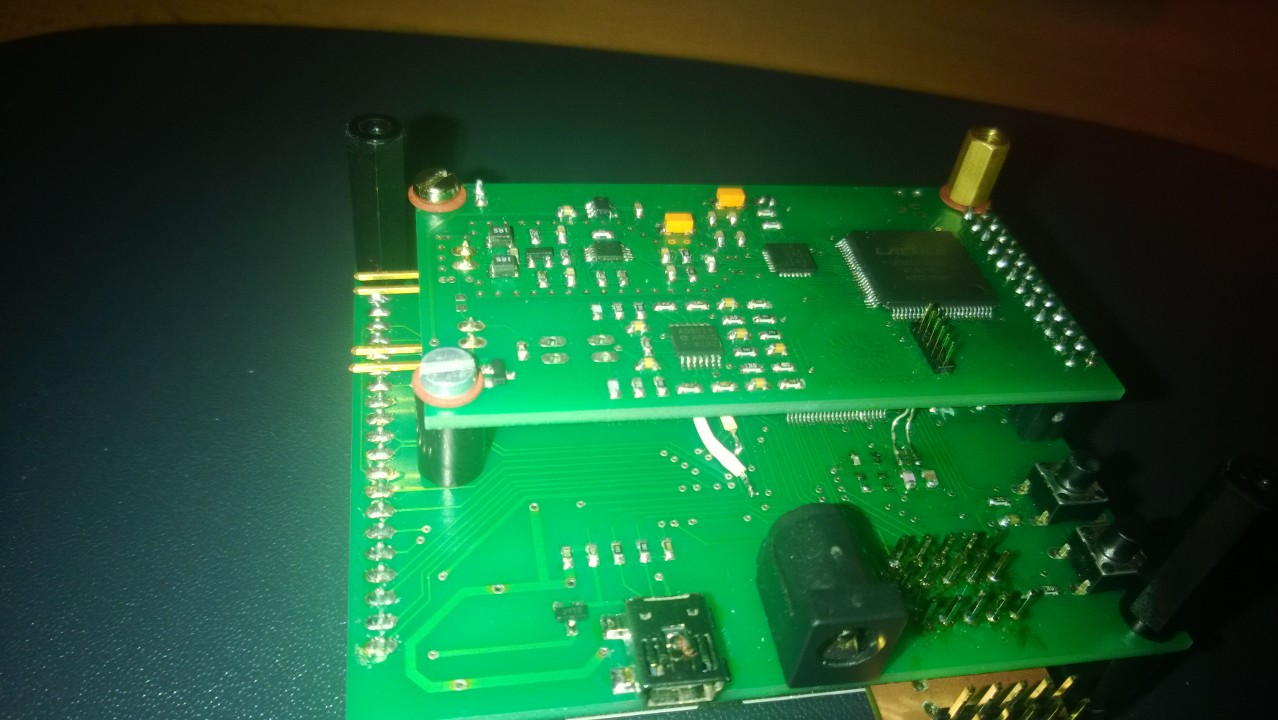
\includegraphics[trim = 10cm 0cm 2cm 5cm, clip=true, width=\textwidth]{systemV2}  
	\caption{Systemaufbau Thesis Rehn}
  	\label{fig:system_stemp}
\end{figure}
\begin{table}[h]
\centering
\caption{Bestandteile der Platine}
\label{tab:system_stemp_tab}
\begin{tabular}{c|l}
\textbf{Nr.} & \textbf{Beschreibung} \\
\cline{1-2}
1 & \ac{cpld} mit Signalerzeugung und Demodulation\\ 
2 & Receiver mit Vorverstärker und \ac{adc}\\
3 & Transmitter mit Differenzverstärker und Übertrager\\
4 & Interface TFT LCD-Display\\
5 & \ac{mcu} mit \ac{usb}-Kommunikation\\
\end{tabular}
\end{table}
%
%
%
\newpage
\subsection{Anforderungen an das Messsystem}\label{sec:anforderungen}
Es werden drei Ebenen von Anforderungen unterschieden: die Benutzeranforderungen, die Systemanforderungen und die Software- und Hardwareanforderungen.\newline
Benutzer und deren Anforderungen werden dabei als höchste Ebene angesehen, da sie die Bedürfnisse des Kunden an das System darstellen. Darunter werden sowohl grundlegende Anforderung, Basisanforderungen sowie Begeisterungsfaktoren beschrieben, welche entschlüsselt, gegliedert und anschließend strukturiert werden müssen.\\
Die grundlegenden Anforderungen, welche Richtlinien und Normen beinhalteten, müssen erfüllt sein. Basisanforderungen beschreiben die Funktionalität des Systems. Nur wenn grundlegende, sowie Basisanforderungen erfüllt sind, kann das System zertifiziert, auf den Markt gebracht und dem Kunden die Möglichkeit gewährt werden, das Produkt zu kaufen. Begeisterungsfaktoren sind Anforderungen, die aus Sicht des Kunden nicht unbedingt erfüllt sein müssen um das Produkt zu kaufen. Jedoch bewegen genau diese Faktoren den Kunden, das Produkt zu kaufen, da es sich durch diese von Konkurrenzprodukten abheben kann. Benutzeranforderungen enthalten derweil keinerlei technische Vorgaben.\newline
Systemanforderungen bilden die mittlere Anforderungsebene, welche die allgemeinen Leistungen des Produktes spezifiziert. Diese Leistungen dienen als Grundlage des Systemdesigns.\newline
Die Software- und Hardwareanforderungen werden aus dem Systemdesign abgeleitet und detaillierter beschrieben.\newline % wodurch die Software- und Hardwaredesign abgeleitet werden.\newline
Bindende und optionale Anforderungen können anhand der Kundenformulierung unterschieden werden. Dabei werden bindende Anforderungen durch "'soll"' oder "'darf nicht"' hervorgehoben. Normativ bindende Anforderungen werden durch "'muss"' Formulierungen dargestellt. Eine optionale Anforderung wird dabei durch "'sollte"' und eine Zusatzfunktion mit "'kann"' formuliert.\newline
Die in dieser Arbeit durchgeführte Optimierung wurde durch die folgenden Anforderungen detailliert definiert.
\subsection*{Benutzeranforderungen}
\begin{itemize}\itemsep0pt
\item Das bestehende USD-System soll aus einer Messplatine bestehen.
\item Das System soll mit Ultraschallsonden im Frequenzbereich von 2, 4 und 8 \ac{mhz} arbeiten.
\item Für eine \ac{prf} sollen mindestens 40 Werte (20 Real-, 20 Imaginärteil) zu Verfügung gestellt werden, um weitere Analysen zu ermöglichen.
\item Das System soll über eine \ac{pc} Software betrieben werden können.
\item Die \ac{pc} Software soll auf den Betriebssystemen Linux und Windows funktionieren.
\end{itemize}
\subsection*{Systemanforderungen}\label{sec:sysreq}
\begin{itemize}\itemsep0pt
\item Das System soll über eine externe Spannungsversorgung betrieben werden, welche den Normen entspricht.
\item Das System soll als Steuereinheit einen ARM-Cortex M4 besitzen.
%\item Das System soll einen funktionsfähigen Audioausgang besitzen.
%\item Das System sollte einen Composite-Out Ausgang besitzen.
\item Das System soll einen USB-micro Anschluss besitzen.
%\item Die Messplatine soll einen Triggerausgang für die Zertifizierung von Ultraschallsonden bereitstellen.
%\item Das System soll einen separaten Ausgang sowie Eingang für Messungen bereitstellen, welche leicht miteinander verbunden werden können.
\end{itemize}
\subsection*{Software- und Hardwareanforderungen}
\begin{itemize}\itemsep0pt
	\item \textbf{Energieversorgung}
	\begin{itemize}\itemsep0pt
		\item Das System soll die Hardware des Energieversorgers vor Fehlfunktionen des Systems schützen.%vor was? Je nach detaillierter Anforderung kann das ziemlich aufwändig werden. Wie würdest Du die Hardware z.B. vor einem Flugzeugabsturz schützen?
		%\item Das System sollte eine maximale Leistungsaufnahme von 2.5W bei 5V DC besitzen.
		\item Das System soll mit einer maximalen Eingangspannung von 20V betrieben werden können.
		\item Das System soll aus der angelegten Spannung die für das System benötigten Spannungen erzeugen.
	\end{itemize}
\end{itemize}
\begin{itemize}\itemsep0pt
	\item \textbf{Messelektronik}
	\begin{itemize}\itemsep0pt
		\item Die Messelektronik soll eine Spannungsversorgung von 3,3 V besitzen.
%		\item Die Messelektronik soll separat aus einer Platine bestehen.
%		\item Ein Trigger Signal sollte vorhanden sein, um das Zertifizierungsverfahren der Sonden und des Systems zu ermöglichen.
		\item Die Messelektronik sollte den \ac{emi} Richtlinien entsprechen.
		\item Die Messelektronik sollte einen Schutz vor zu großen Signalamplituden besitzen.
		\item Die Messelektronik soll eine \ac{prf} von 2 kHz bis zu 12 kHz und eine Abtastrate von 64 MHz besitzen.
		\item Die Platine soll eine steckbare Verbindung für die Sonde aufweisen.
		\item Die Messelektronik sollte über eine Codierung die Frequenz der angeschlossenen Sonde erkennen können.
	\end{itemize}
\end{itemize}
\begin{itemize}\itemsep0pt
	\item \textbf{Auswerteelektronik}
	\begin{itemize}\itemsep0pt
		\item Die Auswerteelektronik soll eine Schnittstelle zu einen \ac{pc} besitzen, welche mindestens eine Datentransferrate von 100 Mbit/s unterstützt.
		\item Eine Visualisierung der aktuell angeschlossenen Sonde mit deren Frequenz sollte vorhanden sein, um den Nutzer eine schnelle Identifizierung der Sonde zu ermöglichen.
	\end{itemize}
\end{itemize}
\begin{itemize}\itemsep0pt
	\item \textbf{\ac{gui}}
	\begin{itemize}\itemsep0pt
		\item Das \ac{gui} soll ein Menu bereitstellen, um die Parameter der Messung einzustellen.
		\item Das \ac{gui} soll ein linearen, für die Messwerte und ein \ac{fft}-Graphen, für das Zeit-Schallsignal bereitstellen.
	\end{itemize}
\end{itemize}
%
%
%
\section{Beschreibung der Methodik}
Die Ausgangssituation wurde analysiert und mit dem aktuellen Stand der Forschung verglichen, indem die zur Verfügung stehenden Unterlagen studiert und mit aktueller Fachliteratur abgeglichen wurden. Durch die Recherchen des aktuellen Stands der Technik zeigte sich entsprechendes Optimierungspotenzial im Vergleich zu den vorhandenen Messsystemen. Insbesondere zeigte sich, dass eine deutliche Verbesserung der Nutzbarkeit erreicht werden kann, wenn eine Datentransfersteigerung des Systems erreicht werden kann. Desweiteren ergab sich Optimierungspotential in der Messgenauigkeit. Durch die Anpassung der Hard- und Software und der Anpassung des Layouts unter Beirücksichtung gängiger \ac{emi} Aspekte, wurden im Rahmen der hier beschriebenen Studienarbeit grundlegend Verbesserungen im Hinblick auf die Genauigkeit der Messung und des Nutzungskomforts des Messystems erreicht.